
	% filters
\subsection{Filters}

\begin{frame}
	\frametitle{Filters}
	\begin{itemize}
		\item several \textbf{filter families:} Butterworth, Chebyshev, elliptic, \ldots
		\item general \textbf{filter types:} low-pass, high-pass, band-pass, band-stop (notch)
		\item \textbf{cutoff frequency} at which output power is reduced by $-3\,\textrm{dB}$ (approx. one half)
		\item \textbf{example:} \texttt{matlab/filters.m}
			\begin{figure}
				\centering
				\begin{subfigure}[c]{0.48\linewidth}
					\cfbox{neutral}{\includegraphics[width=\linewidth]{images/filters_high.eps}}
				\end{subfigure}
				\hspace{0.01\linewidth}
				\begin{subfigure}[c]{0.48\linewidth}
					\cfbox{neutral}{\includegraphics[width=\linewidth]{images/filters_low.eps}}
				\end{subfigure}
			\end{figure}
	\end{itemize}
\end{frame}

\begin{frame}
	\frametitle{Filters}
	\begin{itemize}
		\item filters are represented by feedforward and feedback \textbf{filter coefficients} $b_j$ and $a_j$
		\item high \textbf{filter order} $n$ increases computational complexness but thereby quality
			\begin{align*}
				y_i=\overbrace{\frac1{a_1}\Bigg(\underbrace{\sum_{j=0}^nb_{j+1}x_{i-j}}_{\textrm{FIR}}-\sum_{j=1}^na_{j+1}y_{i-j}\Bigg)}^{\textrm{IIR}}
			\end{align*}
		\item \textbf{FIR filters} (finite impulse response) are slow to compute but stable
		\item \textbf{IIR filters} (infinite impulse response) are fast to compute but might be unstable
		\item often used \textbf{additional terms} (images from \url{http://dspguru.com})
			\begin{figure}
				\centering
				\begin{subfigure}[c]{0.48\linewidth}
					\cfbox{neutral}{\includegraphics[width=0.9\linewidth]{images/response.png}}
				\end{subfigure}
				\hspace{0.01\linewidth}
				\begin{subfigure}[c]{0.48\linewidth}
					\cfbox{neutral}{\includegraphics[width=0.9\linewidth]{images/ripple.png}}
				\end{subfigure}
			\end{figure}
	\end{itemize}
\end{frame}

\begin{frame}[fragile]
	\frametitle{Filters}
	\begin{itemize}
		\item \textbf{Butterworth filter} (high-pass, second-order, $100\,\textrm{Hz}$ cutoff)
			\begin{code}
>> n = 2; \color{medium}% filter order
>> cutoff = 100; \color{medium}% cutoff frequency
>> [b, a] = butter( n, cutoff / (fS/2), 'high' );
			\end{code}
		\item \textbf{Chebyshev filter} (high-pass, $1\,\textrm{dB}$ ripple, $40\,\textrm{dB}$ attenuation, $100\,\textrm{Hz}$ cutoff)
			\begin{code}
>> cutoff = 100; \color{medium}% cutoff frequency
>> stopband = 90; \color{medium}% stopband frequency
>> ripple = 1; \color{medium}% passband ripple
>> attenuation = 40; \color{medium}% stopband attenuation
>> n = cheb2ord( cutoff / (fS/2), stopband / (fS/2), ripple, attenuation );
>> [b, a] = cheby2( n, attenuation, stopband / (fS/2) );
			\end{code}
		\item \textbf{apply any filter}
			\begin{code}
>> y = filter( b, a, x ); \color{medium}% filter signal x using coefficients a, b
			\end{code}
		\item plot filter response
			\begin{code}
>> [h, f] = freqz( b, a, 512, fS ); \color{medium}% complex filter response
>> plot( f, abs( h ).^2 );
			\end{code}
	\end{itemize}
\end{frame}

\begin{frame}
	\frametitle{Filters}
	\begin{itemize}
		\item comparison of some \textbf{filter families} (image from \url{https://en.wikipedia.org})
			\begin{figure}
				\centering
				\begin{subfigure}[c]{0.7\linewidth}
					\cfbox{neutral}{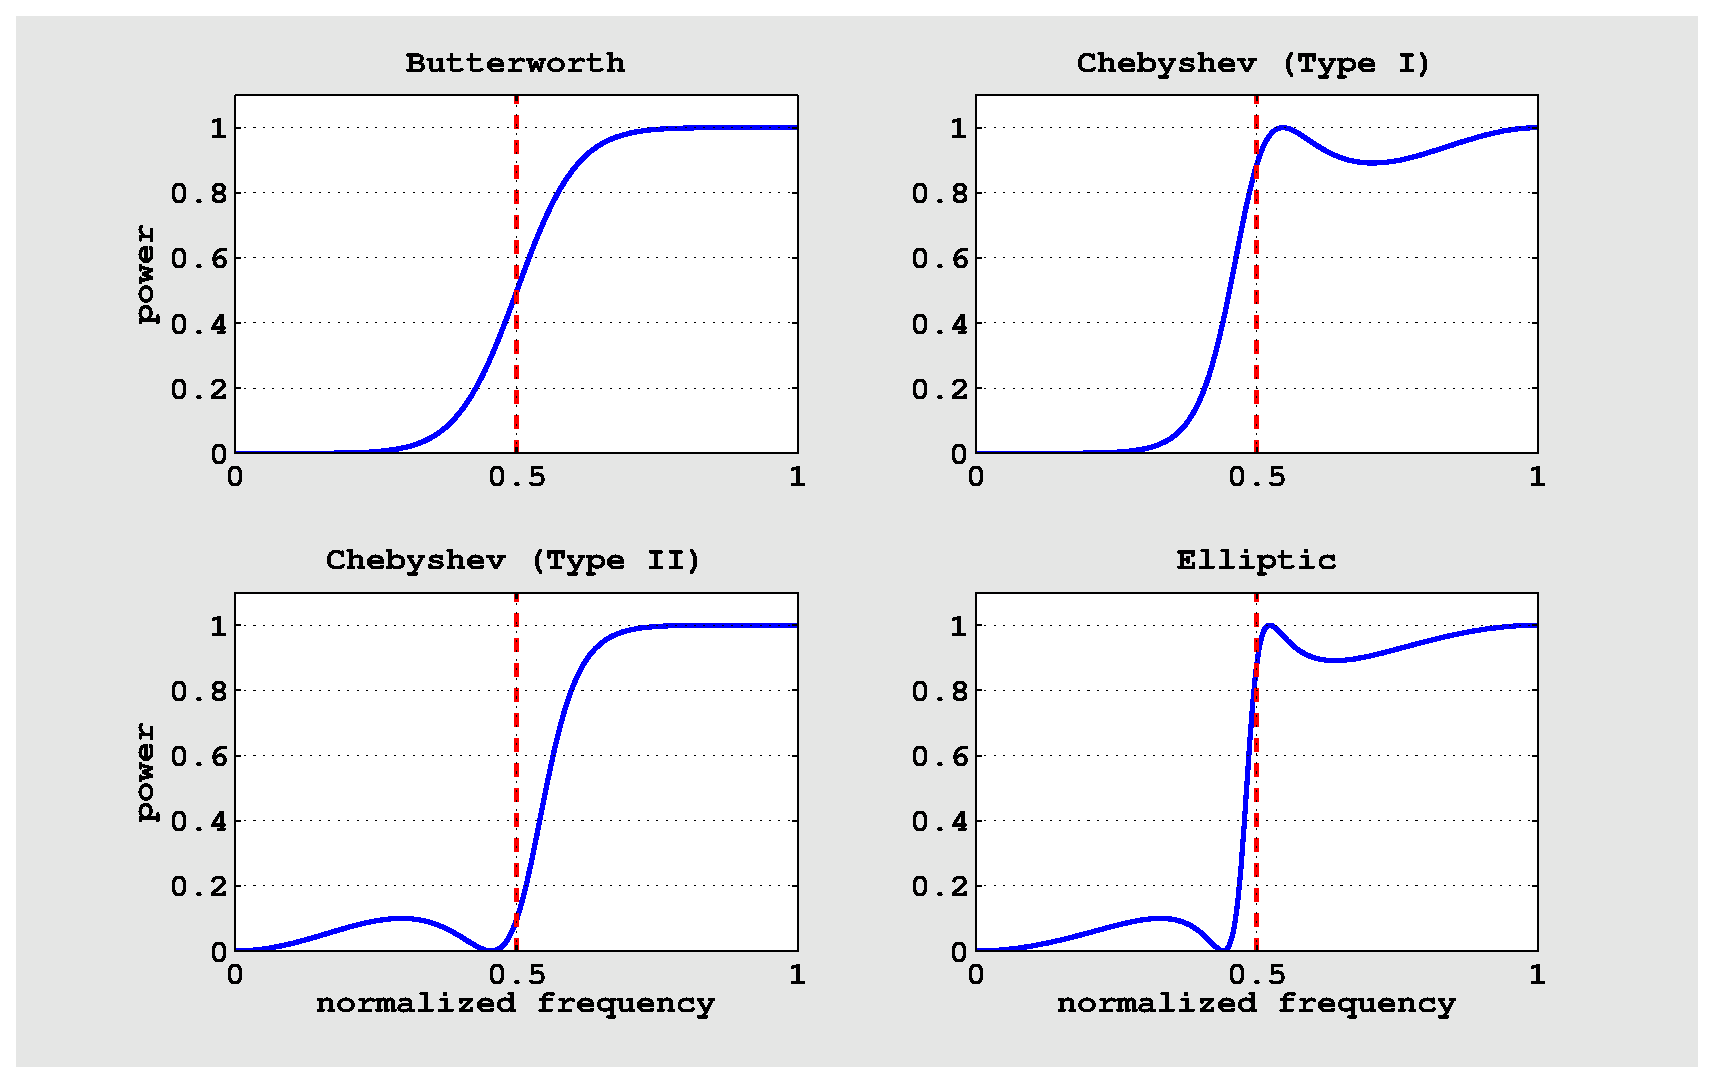
\includegraphics[width=0.9\linewidth]{images/filters.eps}}
				\end{subfigure}
			\end{figure}
		\item \textbf{exercise:} Can you image what \textbf{filter delay} means?
		\item \textbf{exercise:} TODO!
	\end{itemize}
\end{frame}

